\documentclass[12pt]{article} 
\usepackage[utf8]{inputenc}
\usepackage{booktabs}
\usepackage{rotating}
\usepackage{amsthm} % theorems
\usepackage{amssymb}
\usepackage{amsmath}
%\usepackage{framed}
\usepackage{natbib}
\usepackage{graphicx}
\usepackage[]{xcolor}
\usepackage{setspace} %1.5 space
\usepackage[none]{hyphenat} %No hyphenation
%\usepackage[left]{lineno} %Number of lines
\usepackage{float}
%\usepackage{xfrac} %better looking compact fractions
%\usepackage{tikz}
%\usepackage{subfig}
%\usepackage{float}
%\usepackage{booktabs}
\usepackage{hyperref}
\usepackage[nameinlink,noabbrev]{cleveref}
\usepackage{multirow}
\usepackage{array}
%\usepackage{polyglossia}
%\usepackage{blindtext}
\usepackage{colortbl}
%\usepackage[many]{tcolorbox}
%\usepackage{lmodern} 
%\usepackage{caption}
%\usepackage{eurosym}
%\usepackage{pdfpages}r
%\usepackage{standalone} 
\usepackage{pdfpages}
\usepackage{tikz}
\newtheorem{definition}{Definition}
\usetikzlibrary{calc}
\usepackage{amssymb}
\usepackage{amsmath}
\usepackage{array}
\usepackage{graphicx}
\usepackage{booktabs}
\usepackage{rotating}
\usepackage{array}
\usepackage{graphicx}

\usepackage{bookman}

%Luciano to make nice inverted quotes
%\usepackage [autostyle, english = american]{csquotes}
%\MakeOuterQuote{"}
\newcolumntype{L}[1]{>{\raggedright\let\newline\\\arraybackslash\hspace{0pt}}m{#1}}
\newcolumntype{C}[1]{>{\centering\let\newline\\\arraybackslash\hspace{0pt}}m{#1}}
\newcolumntype{R}[1]{>{\raggedleft\let\newline\\\arraybackslash\hspace{0pt}}m{#1}}


\title{Evolution of Conditional Cooperation in Prisoner's Dilemma\footnote{Scripts for the simulations are available on the GitHub repository: \url{https://github.com/seyhunsaral/evolutioncc}}}


\author{Ali Seyhun Saral\thanks{Max Planck Institute for Research on Collective Goods, Bonn, Germany.}}  
\date{August 2020}
\begin{document}
\onehalfspacing
\sloppy
\maketitle        
\begin{abstract}

\thispagestyle{plain}

In this study, we investigate conditional types and their evolution in an iterated Prisoner's Dilemma, comparing different continuation probabilities, by using a computational model. In our setting, agents are characterized by their responses to each level of cooperation in a linearly extended Prisoner's Dilemma. By using repeated simulations, we estimate the likelihood of cooperation and the conditional strategies that are likely to succeed. 

Our results show that, when the continuation probability is sufficiently large, full cooperation is achieved. In this case, the most successful strategies are the ones who employ an all-or-none type of conditional cooperation, followed by perfect conditional cooperators. In the intermediate levels of continuation probability, however, \textit{hump-shaped} contributor types are the ones that are most likely to exist, followed by imperfect conditional cooperators. Those agents cooperate in a medium level of cooperation within themselves and each other. 

Our results provide an explanation for the commonly observed hump-shaped strategy and imperfect conditional cooperators in experiments. Furthermore, a potential implication of our results is that the heterogeneity of conditional strategies might stem from the diverse interaction frequencies among real-world interactions. 

\textbf{Keywords}: reciprocity | conditional cooperation | reactive strategies | hump-shaped contributors 
\end{abstract}

\section{Introduction} 
Humans are distinct in their cooperation capability, if not unique \citep[See][]{Bowles2011,Wilson2012}. As a species, we heavily depend on the mutual cooperation of individuals. At first glance, from an evolutionary perspective, it seems counter-intuitive for  individuals to care for the others: if everybody is cooperating in a population, any fraction of selfish individuals would do better than those who care, and would therefore have a higher evolutionary fitness. As it would be easy to exploit the cooperators in such a population, it is just matter of time for cooperation to be eradicated. Then, how come cooperation is so common in some species including us humans?

 Several explanations have been put forward to explain this puzzle.\footnote{See \citet{Nowak2006} for a summary of some of these mechanisms.} One of the most prominent answers has been reciprocal altruism. The earliest systematic thoughts on the evolution of reciprocal altruism can be found in the writings of the Russian thinker Kropotkin in the early 20th century. In his book \textit{Mutual Aid}, he discusses the evolutionary success of solidarity with some examples from animal groups and human societies in historical perspective \citep{Kropotkin1902-mo}. ``\textit{(...) Natural selection continually must eliminate (anti-social instincts), because in the long run the practice of solidarity proves much more advantageous to the species than the development of individuals endowed with predatory inclinations}'', he asserts \citep[p.~18]{Kropotkin1902-mo}. His arguments today can be interpreted as a mixture of different mechanisms such as reciprocal altruism, group selection and kin selection. It was not until more than half a century later that the biologist Robert Trivers coined the term \textit{reciprocal altruism} and explained its role in the context of cooperation by way of a formal model \citep{Trivers1971}. By using Hamilton's methodology of kin selection \citep{Hamilton1964}, Trivers showed that, given that there is a positive probability for individuals to interact again, if the benefit of an aid is sufficiently greater than its cost, then cooperation of unrelated individuals can arise. Trivers's treatise on reciprocity has been highly influential, especially in the field of theoretical biology. 

In game theory literature, Folk theorems show that, if the threat of defection is present in the future, cooperating today is more beneficial; therefore, a cooperative strategy in the stage game, as well as any other individually rational strategy, can be the equilibrium of the supergame \citep{Friedman1971-nz, Fudenberg1986-dz}. In addition to that, \citeauthor{Axelrod1980a}'s simulations on the Prisoner's Dilemma  support those theoretical results by showing that the reciprocal \textit{tit-for-tat} is a strong strategy that allows cooperation while it is immune to exploitation by selfish players \citep{Axelrod1980a,Axelrod1980b,Axelrod1981-ot}. 

With these scientific accounts, a rather optimistic picture of cooperation through reciprocity has been drawn. The main dynamics of cooperation through reciprocity can be summarized as follows: reciprocators cooperate among each other as they reciprocate kindness over time. Therefore they receive a higher payoff than the selfish types who meet other selfish types. And when a reciprocator meets a selfish type, the reciprocator responds selfishly after the first defection. Thus, the exploitation of a reciprocator by a selfish individual is not sustainable when the probability of continuation is sufficiently high. 

Nevertheless, with the rise of experimental economics, empirical evidence on the Prionser's Dilemma and the Public Goods Game draws a rather different picture: the contributions tend to decline over time, whether subjects play the game within the same group or matched with others \citep{Selten1986-uc, Andreoni1993-ys, Cooper1996-be, ledyard1994public, Kim1984-wm, Isaac1985-qz, Andreoni2008-ec}. This declining trend in the Public Goods Game is often, and arguably best, explained by conditional preferences. Clear evidence is provided by \citet{Fischbacher2001}, who collects conditional choices of subjects to the common pool by using the strategy method. According to their results, most of the participants reveal a preference pattern, in which they will only contribute if the others contribute as well, albeit with a \textit{selfish bias}; they tend to contribute less to the public pool than the others. Those type of conditional cooperation is not sufficient to sustain cooperation, as contributions tend to decline over time\citep{Fischbacher2010}.

In this study, we aim to investigate the conditional preferences in the framework of \citet{Fischbacher2001}, using computational methods. We examine the evolutionary success of those conditional strategies in a social dilemma with a simplified framework.  We create populations of agents with the types drawn from of the set of all conditional strategies within our framework. Each agent randomly pairs with another agent to interact in this social dilemma, and continues to interact with probability $\delta$. We let an evolutionary reproduction mechanism based on the success of the strategies shape the population structure and we examined success of those strategies for different continuation probabilities $\delta$. 

Our results can be summarized as follows: selfish and close-to-selfish conditional cooperators are likely to be successful when the repetition probability is relatively low. Depending on the value of continuation probability, imperfect conditional cooperators who only fully cooperate when the opponent fully cooperates, perfect-conditional cooperators, and agents with hump-shaped contribution schedule are relatively successful when the repetition probability is sufficiently high. Unconditionally cooperating strategies are unlikely to survive even at high probabilities of repetition. And finally we conclude that the initial move aligned with the conditional strategy plays a crucial role in the survival of those conditional strategies.

\section{Literature Review}

Conditional cooperation has been attracting interest in economics, especially after the seminal work of \citet{Fischbacher2001} who conducted a Public Goods experiment that gave subjects the chance to choose the contribution amount to the public pool according to the average contribution of the others. According to the contribution schedule, they classified subjects as follows: \textit{conditional cooperators}, who increase their contributions with the increasing amount of average contribution of others; \textit{selfish players}, who contribute nothing to the public pool regardless of what others do; and \textit{hump-shaped contributors}, who increase their contribution up to a certain level, most commonly to halfway to the maximum contribution, only to decrease their contributions after that level, as the contributions of others continue to increase. \textit{Unconditional cooperators} were virtually absent in their experiment. Fischbacher, G{\"a}chter and Fehr concluded that most of the subjects are selfish-biased conditional cooperators. In a follow-up study, \citet{Fischbacher2010} showed the dynamics of such contribution patterns, which predict the decline in Public Goods Games. Those conditional strategies defined by Fischbacher can be investigated in the class of reactive strategies, as they only consider the previous move (or, in the simultaneous case, the current move) of the player(s) with whom they interact. 

Possibly because rational and self-interested agents have been central in economic methodology, early models based on conditional strategies were investigated in disciplines other than economics, which employ game-theoretical approaches, such as biology and political science. Axelrod's research showed the success of \textit{tit-for-tat}, a strategy beginning with cooperation in the initial interaction and then copying its opponent's from the previous period \citep{Axelrod1980a, Axelrod1980b, Axelrod1981-ot}.  A tit-for-tat strategy in a Fischbacher-G{\"a}chter framework would be  equivalent to a perfect-conditional-cooperation strategy that matches the individual's contribution to the contribution by others. One should expect this kind strategy to be employed in real-life decisions due to the success of tit-for-tat strategy. In the experiments, however, perfect-conditional-cooperators are outnumbered by imperfect conditional cooperators who tend to give less than what others give. Reciprocity by imperfect conditional cooperators not enough to sustain cooperation, not just within other commonly observed conditional types, but also when they interact among each other \citep{Fischbacher2010}.  Moreover, later results showed that the tit-for-tat strategy was vulnerable when mistakes happen: when an accidental decline occurs, tit-for-tat was not able to reestablish cooperation back again, unless another mistake corrected it \citep{Hirshleifer1988-fh, Selten1984-sb, Fundenberg1990-up, Nowak1993-gl}.


A related line of research with conditional strategies was mostly investigated in biology. So-called ``variable investment models'' provided more insights into successful conditional-like strategies in social dilemmas. These models differ considerably from conditional strategies defined in a Fischbacher-G{\"a}cther framework, as well as from each other by their assumptions; therefore it is not straightforward to compare their results.\footnote{See \citet{Sherratt2002-lx} for a review of some early papers.} For instance,  in \citet{Doebeli1998-cw}, the agents are characterized by two parameters; a parameter that defines the unconditional altruism, and another defining the amount of reciprocation proportional to the difference between one's own altruism and that of the other. In their setup, they use a continuous altruistic investment game in which the marginal benefit of altruism  decreases.  Their evaluation of the success of their strategies takes pairwise comparison into account with the mutants of that strategy. They show that, unless a spatial structure is assumed, selfish types are the most successful ones. \citet{Roberts1998-es} use a different agent definition in which costs and benefits are linear and investments can increase. They take representative strategies for a tournament: \textit{Non-altruistic} agents, who do not invest at all; \textit{Give-as-good-as-you-get} strategies, which invest as much as the other; \textit{raise-the-stake} strategies, amplifying the investment, \textit{short-changer} strategy, which gives less to the other than what the other gives, \textit{all-or-nothing} strategy, which gives an amount and amplifies it only if other reciprocates as much or more. Roberts and Sheratt find that the raise-the-stake strategy is a stable cooperator as it cautiously invests but repeated interactions allow it to reach high cooperation levels.

\citet{Wahl1999-zi,Wahl1999-nn} provide a framework of reactive strategies under adaptive dynamics by providing a linear and continuous extension of the Prisoner's Dilemma in which different amount of contributions are possible. In their framework, they define a reactive strategy with three parameters: the initial move, the slope of the reaction function, and the intercept of the reaction function. Their results suggest that the initial move is a decisive factor in terms of success of a strategy. Moreover, Wahl and Nowak conclude that strategies that are generous, uncompromising and optimistic (in terms of initial move) are the most successful ones. An important result of those studies is  that they demonstrate cycles of cooperation and defection over time. Indirect invasions deter reciprocal strategies which are normally resistant to direct invasion: more cooperative and/or compromising strategies are able to invade reciprocal strategies as those types are exploitable. That allows the invasion of the population by selfish types. 
% I obviously need to add some other stuff here and connecting the paragraph below. 
%The oscilations between cooperation and defection has been a commonly observed result in different theoretical and computational studies of prisoners dilemma game and variants as there is no evolutionary stable pure strategy in prisoners' dilemma game \citet{Nowak1989-vx, Bendor1995-zf, Imhof2005-ti, Van_Veelen2012-xf}. 
% The parallelism of those strategies are notable with the \citet{Fischbacher2001} type of strategies, give-as-good-as-you-get resembles a perfect conditional cooperator, while short-changer resembles an imperfect conditional cooperator.

\citet{Van_Veelen2012-xf} uses a generalized computational model. They run simulations of a Prionser's Dilemma game with finite automata. Their strategies can evolve to be reactive strategies or strategies that consider several rounds of histories depending on the complexity of the strategy generated by mutations. Moreover, their model investigates different levels of assortativity in the population structure. They show that reciprocity and population structure can jointly work in favor of reciprocal strategies. However, reciprocity itself is not sufficient to create and to foster cooperation with random interactions. 

Considering these theoretical and computational results on conditional cooperation and reactive strategies, the following question arises; if we consider the set of strategies with those conditional strategy classifications defined by \citet{Fischbacher2001} framework, how likely would it be for cooperation to arise, and which particular strategies would be more successful than the others?

The two closest approaches to our study are \citet{Szolnoki2012-zq} and \citet{Zhang2016-pz}. \citet{Szolnoki2012-zq} use a spatial structure to investigate conditional cooperation in Public Good Games. Their agents condition on the number of cooperators rather than the strategies themselves. The authors found that the more cautious conditional cooperators enable high levels of cooperation and limit the outreach of defectors by surrounding them spatially. And a recent paper by \citet{Zhang2016-pz} investigates the evolution of conditional types in a Public Goods Game in an agent-based model. The strategies their agents use are a combination of continuous and discrete functions. In authors' setup, a multilevel selection procedure is used. They found that the most successful type is the conditional cooperator type that contributes nothing up to a mid-level contribution by others, but increases its contribution gradually to the full cooperation when others agents' average contribution is maximum. This type of strategy can be considered as ``all-or-nothing'' type of strategy. 

As we draw the general picture, there are certain regularities and mixed results in the literature. Those related with our research questions can be summarized as the following:

\begin{itemize}
    \item Cooperation and defection strategies are likely to oscillate in most settings, especially without certain assumptions in the population structure. In Prisoner's Dilemma game, no pure strategy is evolutionary stable, and reactive strategies are vulnerable to indirect invasions.\citep{Van_Veelen2012-ch, Van_Veelen2012-xf} Therefore, those strategies that use a mixture of actions need further investigation.

\item When there is room for mistakes, it is often unclear how the results obtained by simulations align with theoretical expectations.

\item There is a certain degree of mismatching between the actual behavior in experiments and the theoretical predictions in the framework of conditional strategies.
 
\end{itemize}

Therefore our study aims to fill this gap by demonstrating the success and estimating the likelihood of conditional strategies.

\section{Methods}

Our model has certain differences compared to those models in the literature which we referred in the previous section. First, we choose a setup that is closer to a standard economics framework, in the sense that we do not assume a population structure, but instead use uniform random matching procedure for our agents. However our simulations can easily be extendable to such population structures. Second, we use a minimal setup which allows us to observe conditional strategies, ad defined by Fischbacher \& G{\"a}chter framework, and which avoids unnecessary computational complexities. We use an iterated Prisoners Dilemma with three strategies and discrete linear response functions that do not assume or limit the shape of our response functions. Moreover, we also control for the initial reactions, as it is often stressed that they play an important role on the path of the dynamics. In this section, we start by explaining the social dilemma framework we use, and then we give details of the evolutionary model we use. And we finally describe the outcome variables we are interested in. 

\subsection{Linear Extension of the Iterated Prisoner's Dilemma} 
 We use an extension of the Prionser's Dilemma game Three-Actions Sequential Prisoner’s Dilemma (3SPD) \citep{andreozzi2020stability}. In this extended game, the three actions represent different cooperation levels: $L$(Low) refers to no cooperation/defection; $M$(Medium) refers to an intermediate cooperation level; and $H$(High) refers to full cooperation.  

The cost of cooperation is $c$, while the benefit of cooperation to the opponent is $b$, with the constraint $b>c>0$. If an agent plays the strategy $L$, he keeps his endowment for himself and no change will occur in payoff of the opponent. If agent plays the strategy $H$, he pays the cost $c$ and his opponent gets the benefit $b$. If the player plays $M$, he will only pay the half the amount of the cost of full cooperation but the benefit to the opponent will be half as much as well, i.e., the agent pays a cost of $c/2$, while the opponent gets the benefit $b/2$. 

If the agents were to decide simultaneously, the game matrix would be as shown in \Cref{tbl:evo-game-normal}. For our simulations, we used the following parameters: the cost of cooperation $c$ is equal to 1, the benefit of cooperation $b$ is equal to 2, and we set the base payoff to $1$ to avoid negative payoffs. The normal-form representation of the game with those parameters is shown in \Cref{tbl:evo-game-normal-par}.


\begin{table}[H]
\centering
\setlength{\extrarowheight}{2pt}	\resizebox{0.67\textwidth}{!}{
\begin{tabular}{cc|c|c|c|}
& \multicolumn{1}{c}{} & \multicolumn{3}{c}{Player $2$}\\
& \multicolumn{1}{c}{} & \multicolumn{1}{c}{$L$}  & \multicolumn{1}{c}{$M$} & \multicolumn{1}{c}{$H$}  \\\cline{3-5}
\multirow{3}*{Player $1$}  & $L$ & $(0,0)$ & $(\frac{b}{2},-\frac{c}{2})$ & $(b,-c)$ \\\cline{3-5}
& $M$ &  $(-\frac{c}{2},\frac{b}{2})$ &  $(\frac{b-c}{2},\frac{b-c}{2})$ &  $(b - \frac{c}{2}, \frac{b}{2}-c)$ \\\cline{3-5}
& $H$ & $(-c, b)$ & $(\frac{b}{2}-c,b - \frac{c}{2})$ & ($b-c$, $b-c$) \\\cline{3-5}

			\end{tabular}
		}

\caption[Extended PD]{Extended Prisoner's Dilemma Game}	
\label{tbl:evo-game-normal}
\end{table}


\begin{table}[H]
\centering
\setlength{\extrarowheight}{2pt}	\resizebox{0.67\textwidth}{!}{
\begin{tabular}{cc|c|c|c|}
& \multicolumn{1}{c}{} & \multicolumn{3}{c}{Player $2$}\\
& \multicolumn{1}{c}{} & \multicolumn{1}{c}{$L$}  & \multicolumn{1}{c}{$M$} & \multicolumn{1}{c}{$H$}  \\\cline{3-5}
\multirow{3}*{Player $1$}  & $L$ & $(1,1)$ & $(2,0.5)$ & $(3,0)$ \\\cline{3-5}
& $M$ &  $(0.5,2)$ &  $(1.5,1.5)$ &  $(2.5, 1)$ \\\cline{3-5}
& $H$ & $(0, 3)$ & $(1, 2.5)$ & $(2, 2)$ \\\cline{3-5}

			\end{tabular}
		}

\caption[Extended PD with the Parameters]{Extended Prionser's Dilemma Game with Simulation Parameters $b$=2, $c=1$ and the Base Payoff $1$}	
\label{tbl:evo-game-normal-par}
\end{table}

In order to investigate conditional strategies in terms of the effect reciprocity on cooperation, we used a sequential game setting based on the iterated Prisoner's Dilemma. In our game, for each pair, one of the players is randomly selected as the first mover and makes the initial move. At this point, the agent will bear the cost of his or her action, and the opponent will benefit from this action, if any. 

We use an infitely repeated game approach to the iterated Prisoner's Dilemma Game: After each round, the game continues with the probability of repetition $\delta$. 

In the first round, the first movers start with their initial move. Then if the game continues, second movers respond to what their match did in the previous round according to their conditional strategies. If the game further continues, the first-mover agents in the first round similarly responds to that action with their own conditional strategy. 

\subsection{Conditional Strategies}
In our model, an agent is characterized by his or her conditional strategy. As our extended Prisoner's Dilemma has three possible actions ($L$, $M$ and $H$), a conditional strategy has three components in addition to the initial strategy. We represent each strategy with four letters; the first letter separated from the rest with a hyphen. The first letter corresponds to the initial move of the strategy, where the other three letters denote the conditional responses to $L$, $M$, $H$ respectively. Since, in our context, there are three possible actions for four different situations, in total there are $81$ possible strategies($3^4$). The set of all possible strategies and their classification can be found in \Cref{chap:appx-evo}.

\Cref{fig:evo-stategies}  is a demonstration of two conditional strategies in interaction. The left side shows the actions of the first agent represented by the blue color, while the right side shows the actions of the agent represented by the red color. The blue circle refers to the initial move of the left agent, while the blue arrows, pointing from the actions of the other agent to the player's own actions, represents a conditional reaction. Similarly, for the red agent, the red circle represents the initial movement, and the arrows represent the conditional responses.

	\begin{figure}[H]
\centering
%\documentclass[]{standalone}
%\usepackage{tikz}
%\usetikzlibrary{calc}
%\begin{document}


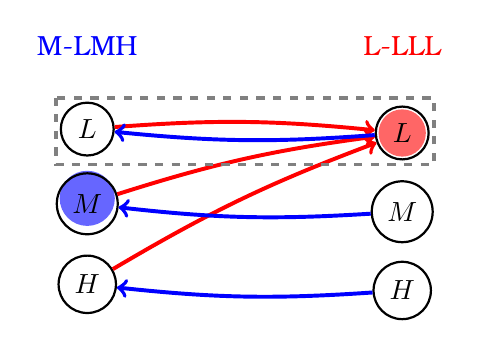
\begin{tikzpicture}
\tikzstyle{dots}=[circle,draw=black,thick]
\tikzstyle{lines1}=[->,line width=0.5mm,red,bend left=5]
\tikzstyle{lines2}=[->,line width=0.5mm,blue,bend left=5]
\tikzstyle{fixedp}=[->,dashed,line width=0.5mm,gray]

\def\arrowhead{10mm}
\fill[red!60,thick,dashed] (4,-1.1) circle (0.3cm);
\fill[blue!60,thick,dashed] (0,-1.93) circle (0.35cm);
\draw[shift={(0,-1.4)},color=black] node[dots,above] (aL){ $L $ };
\draw[shift={(0,-2.4)},color=black] node[dots,above] (aM){ $M $ };
\draw[shift={(0,-3.4)},color=black] node[dots,above] (aH){ $H $ };
\draw[shift={(4,-1.1)},color=black] node[dots] (bL) { $L $ };
\draw[shift={(4,-2.1)},color=black] node[dots] (bM) { $M $ };
\draw[shift={(4,-3.1)},color=black] node[dots] (bH) { $H $ };


\node[text=blue] at (0,0) {M-LMH};
\node[text=red] at (4,0) {L-LLL};
\draw[lines1] (aL) edge (bL);
\draw[lines1] (aM) edge (bL);
\draw[lines1] (aH) edge (bL);
\draw[lines2] (bL) edge (aL);
\draw[lines2] (bM) edge (aM);
\draw[lines2] (bH) edge (aH);
\draw[fixedp] (aL)++(-.4,+.4) rectangle ($ (bL) + (.4,-0.4) $);
\end{tikzpicture}
%\end{document}


		\caption[Demonstration of Interacting Agents]{A Demonstration of the Interaction of Two Agents with Respective Conditional Strategies $M-LMH$ and $L-LLL$}
\label{fig:evo-stategies}
	\end{figure}

As can be seen from the figure, the blue player has the action $M$ as the initial move, and respectively he/she plays $L$ if the opponent plays $L$, $M$ if the opponent plays $M$, and $H$ if the opponent plays $H$. Therefore, this type of the agent is denoted as $M-LMH$. 

To give an example of the interaction, if the blue player is selected as the first-mover, it starts with the action $M$. The red arrow from that node points to action $L$ of the red player, therefore the red player responds with $L$. If the game continues,the blue player responds with $L$ and if it continues further, the red player responds with $L$, and so on. 

\subsection{Computational Model}

In terms of the procedures of population generation, reproduction and mutation, we use a similar methodology with \citet{Van_Veelen2012-xf}. First, we generate a population with a fixed size of 200 agents. The type of the agents in this population are sampled from all 81 possible types. Each agent lives for one generation. In each generation, agents are matched in pairs randomly. After they are paired, the agents play the extended iterated Prionser's Dilemma we described in the previous sections. The interaction is repeated with probability $\delta$. To reduce computational complexity, we sampled the number of interactions from a geometric distribution for each matching in each generation.\footnote{The expected number of interactions for a given $\delta$ is $E[T] = \frac{\delta}{1-\delta}$. As the first interaction occurs with certainity in our setting, the expected number of interactions is $1 +\frac{\delta}{1-\delta} = \frac{1}{1-\delta}.$} For each interaction, we normalize the payoffs by dividing the total payoff by the number of interactions in order to fix the effects of different delta values. After the interaction by two individuals are stopped, we resample the population according to payoffs; each agent is expected the have the offspring in the next generation with the probability that is equal to the proportion to its payoff to the total payoff. Therefore, agent $i \in N$ has the probability of resampling in the next generation $\dot{p}$:

$$ \dot{p}_i  = (\pi_i/\sum\limits_{j \in N}\pi_j)(1-p_M),$$ where $\pi_l$ denotes the normalized payoff of individual $l$, $N$ denotes the set of agents, and $p_M$ denotes the probability of mutation. Each type has the same probability of taking place in the next generation through mutations.

We use Monte-Carlo method for our investigation: We repeat each simulation with the specific parameter for 500 times independently. That allows us to obtain the mean frequency of each action and each strategy in each parameter and generation over the total number of simulations. Then, these frequencies can be interpreted as the probability of an action/strategy to exist in a given parameter. 

\begin{table}[H]
\centering
\begin{tabular}{@{}p{0.2cm}p{5.5cm}l@{}}
\toprule
&Stage     & \hspace{2em} Details  \\ \midrule

& \multirow{2}*{Population Generation}     & Number of Agents: 200 \\
&                                          & Uniformly from all possible types \\ \midrule 
& Matching                                 & Two players: random matching \\ \midrule
& \multirow{2}*{Interaction}               & Extended iterated Prisoners Dilemma  \\
&                                          & Repetition with probability $\delta$ \\ \midrule
& \multirow{2}*{Reproduction and Mutation} & Resampling proportional to normalized payoff\\
&                                          & Uniform random mutation with a fixed probability \\ 
&                                          & Ran for 5000 generations \\ \midrule
& \multirow{2}*{Resampling}                               & Regeneration of the population with the same \\ 
&                               & parameters for 500 times \\ \bottomrule


\bottomrule

\end{tabular}
\caption{Summary of the Computational Stages}
\label{evo:modeldesc}
\end{table}

 In our model, each agent has a probability of making a mistake $p = 0.005$. This means, either as the first mover in the first interaction, in the later interactions, an agent plays a random strategy. Our results show that mistakes we introduce has minor effects on the rate of cooperation. The comparision of the simulation results between the case with mistakes and without them can be seen in \Cref{fig:mistake-comparision}.

 As the repetition probability $\delta$ is the key parameter we are interested in, we covered a range of values from $0.5$ to $0.95$ with increments of $0.05$. The results we have obtained are reported in the next section.

%\subsection{Theoretical expectations}

% Change the picture probably

\section{Results}
\label{sec:results}

%\subsection{Computational Results}
To interpret the results we have obtained, first we start by demonstrating three single instances of our simulations for different delta values. \Cref{fig:evo-actionssingle} shows the fraction of the actions that are being played in each generation, while \Cref{fig:evo-typessingle} shows the distribution of types in the same interaction.   
\begin{figure}[H]
	\centering
	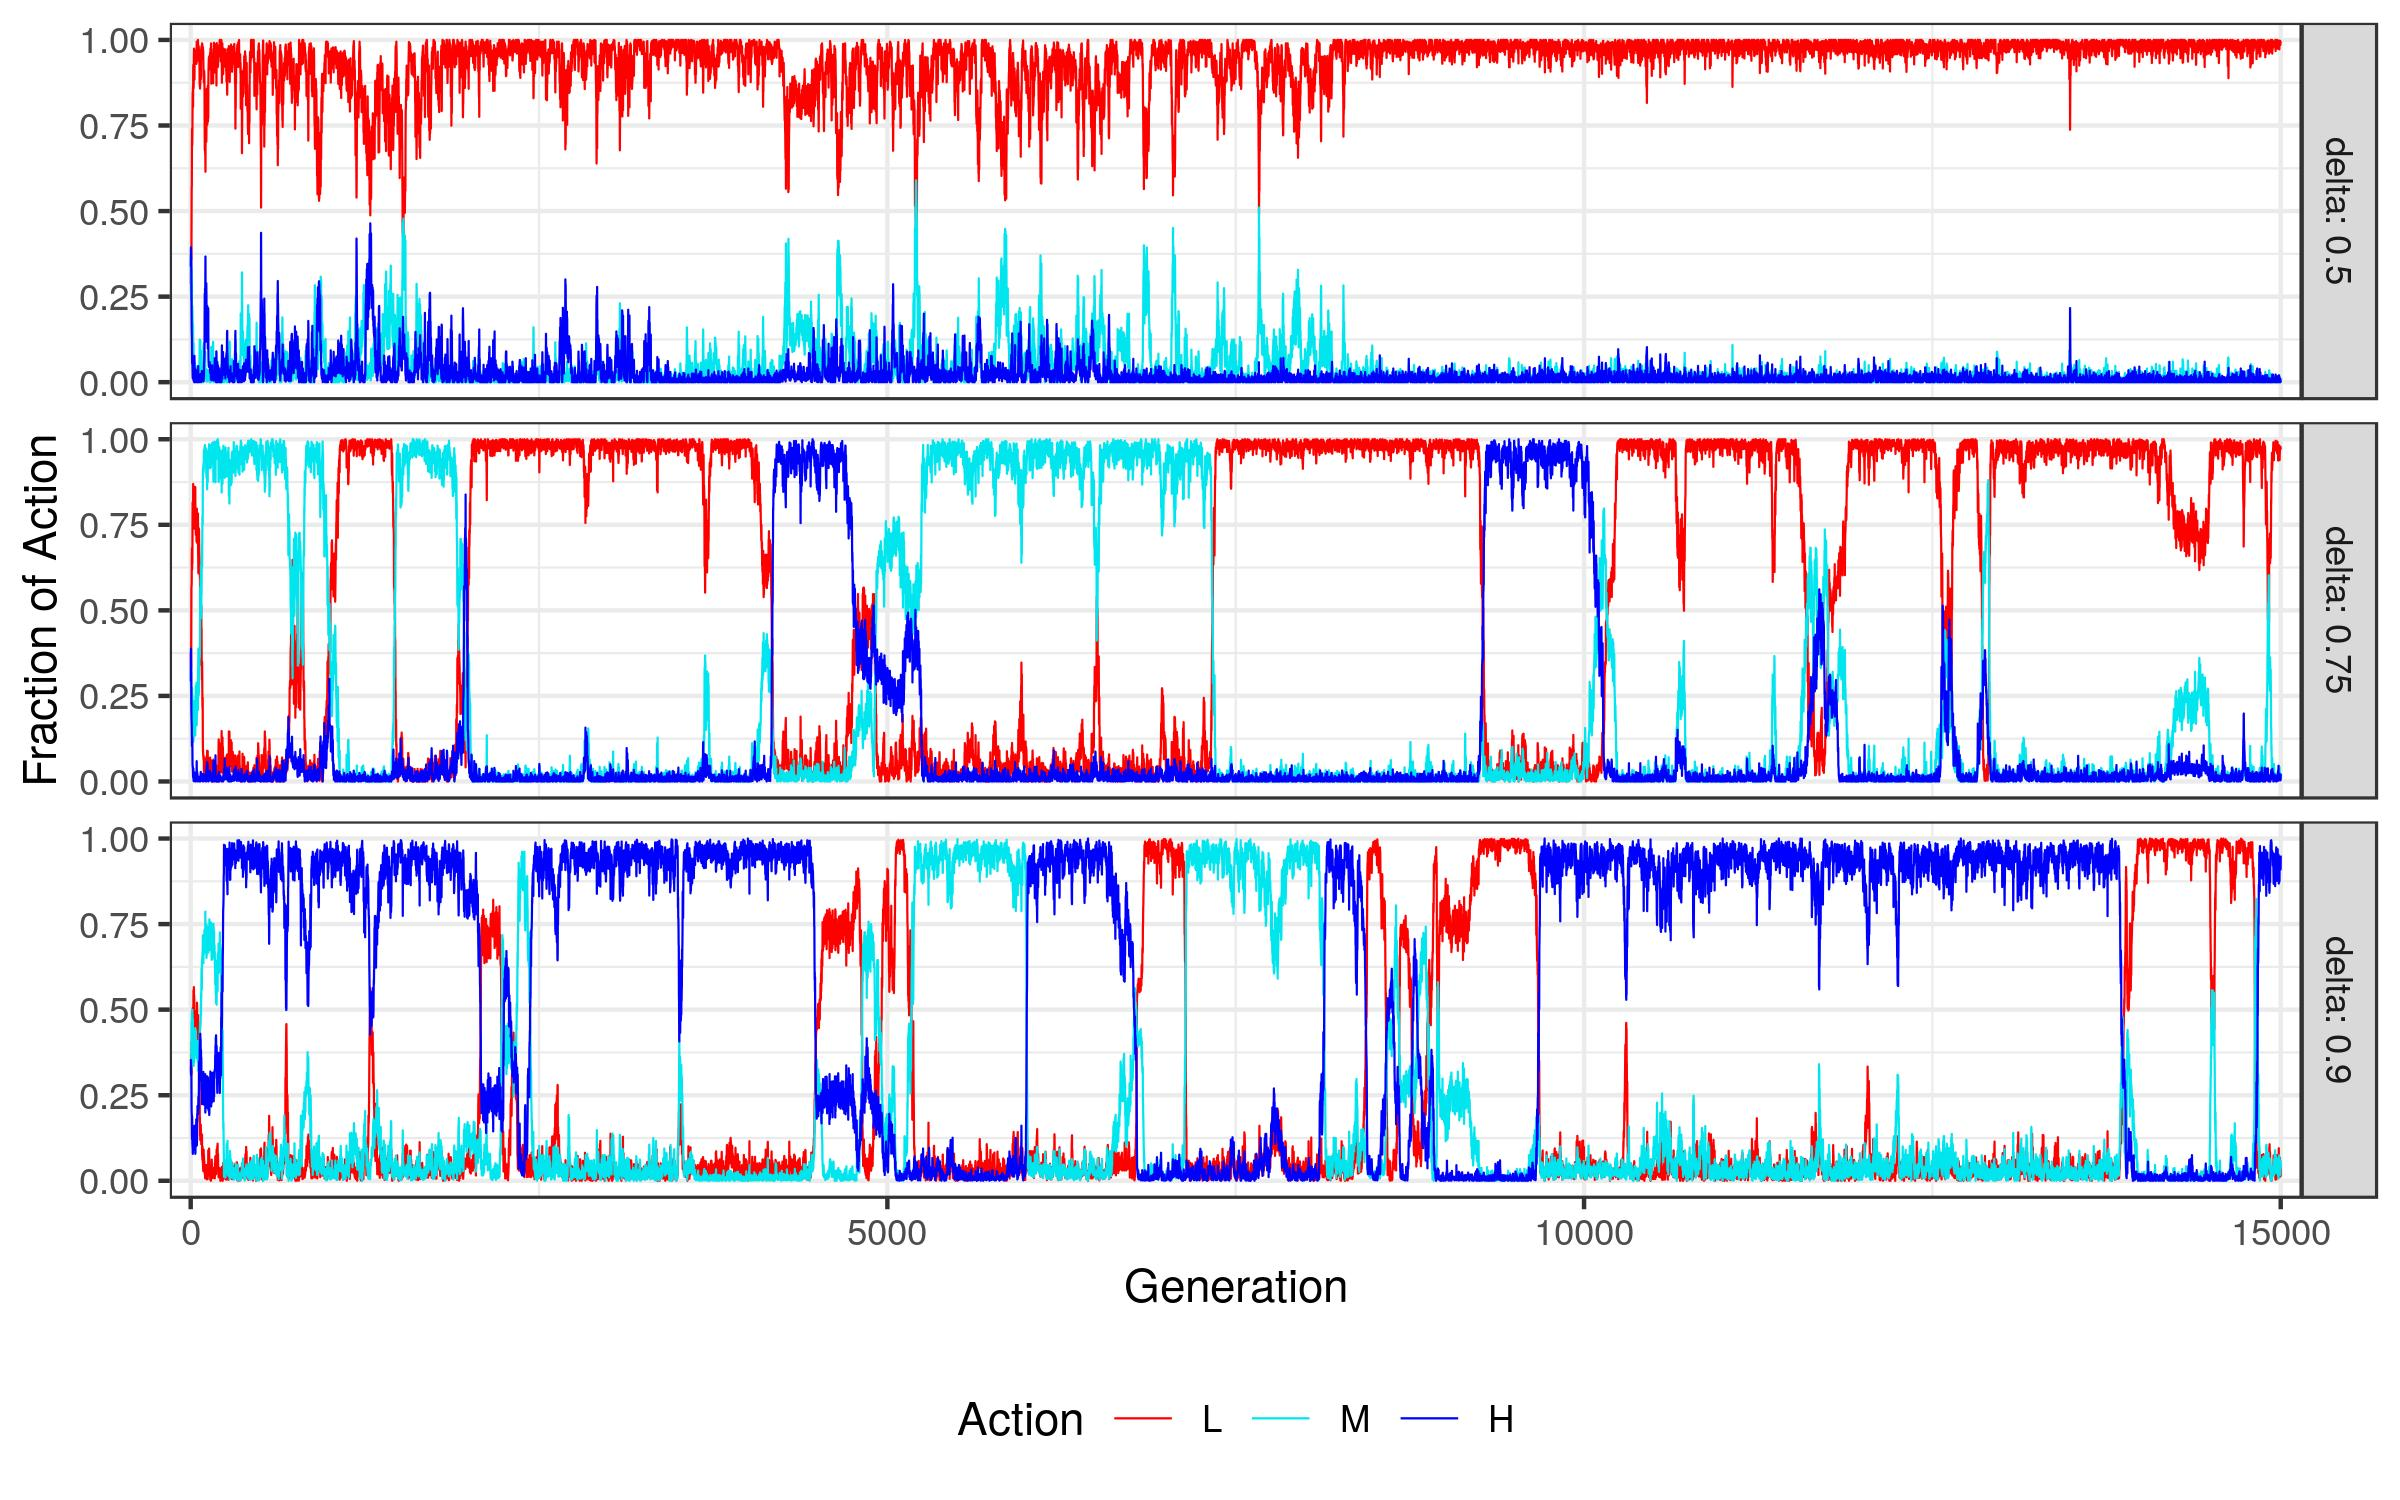
\includegraphics[width=1\linewidth]{img/actions_singlerun2}
	\caption[Fraction of Actions During Three Instances]{Fraction of Actions During Three Instances of Simulation with Different Continuation Probabilities}
	\label{fig:evo-actionssingle}
\end{figure}

 As can be seen from \Cref{fig:evo-typessingle}, no type dominates the population for a long time. However, when $\delta$ is low, defection(L) outperforms cooperative strategies. In this case the types that are taking over the population are neutral mutants of the selfish type. When $\delta$ increases, occasional oscillations occur both in types and also in the actions. A single type takes over the population and stays as the most common type until another type with direct or indirect mutation takes over.  This result is not unexpected, as no type is resistant to indirect invasion in a Prionser's Dilemma \citep{Van_Veelen2012-xf, Garcia2016-tr, Garcia2018-aj}. But it gives us the intuition on how to interpret our result of resampled simulations. As cooperation and defection can occasionally occur, we should interpret our result in a probabilistic way rather than an expected state of a population.
\begin{figure}[H]
	\centering
	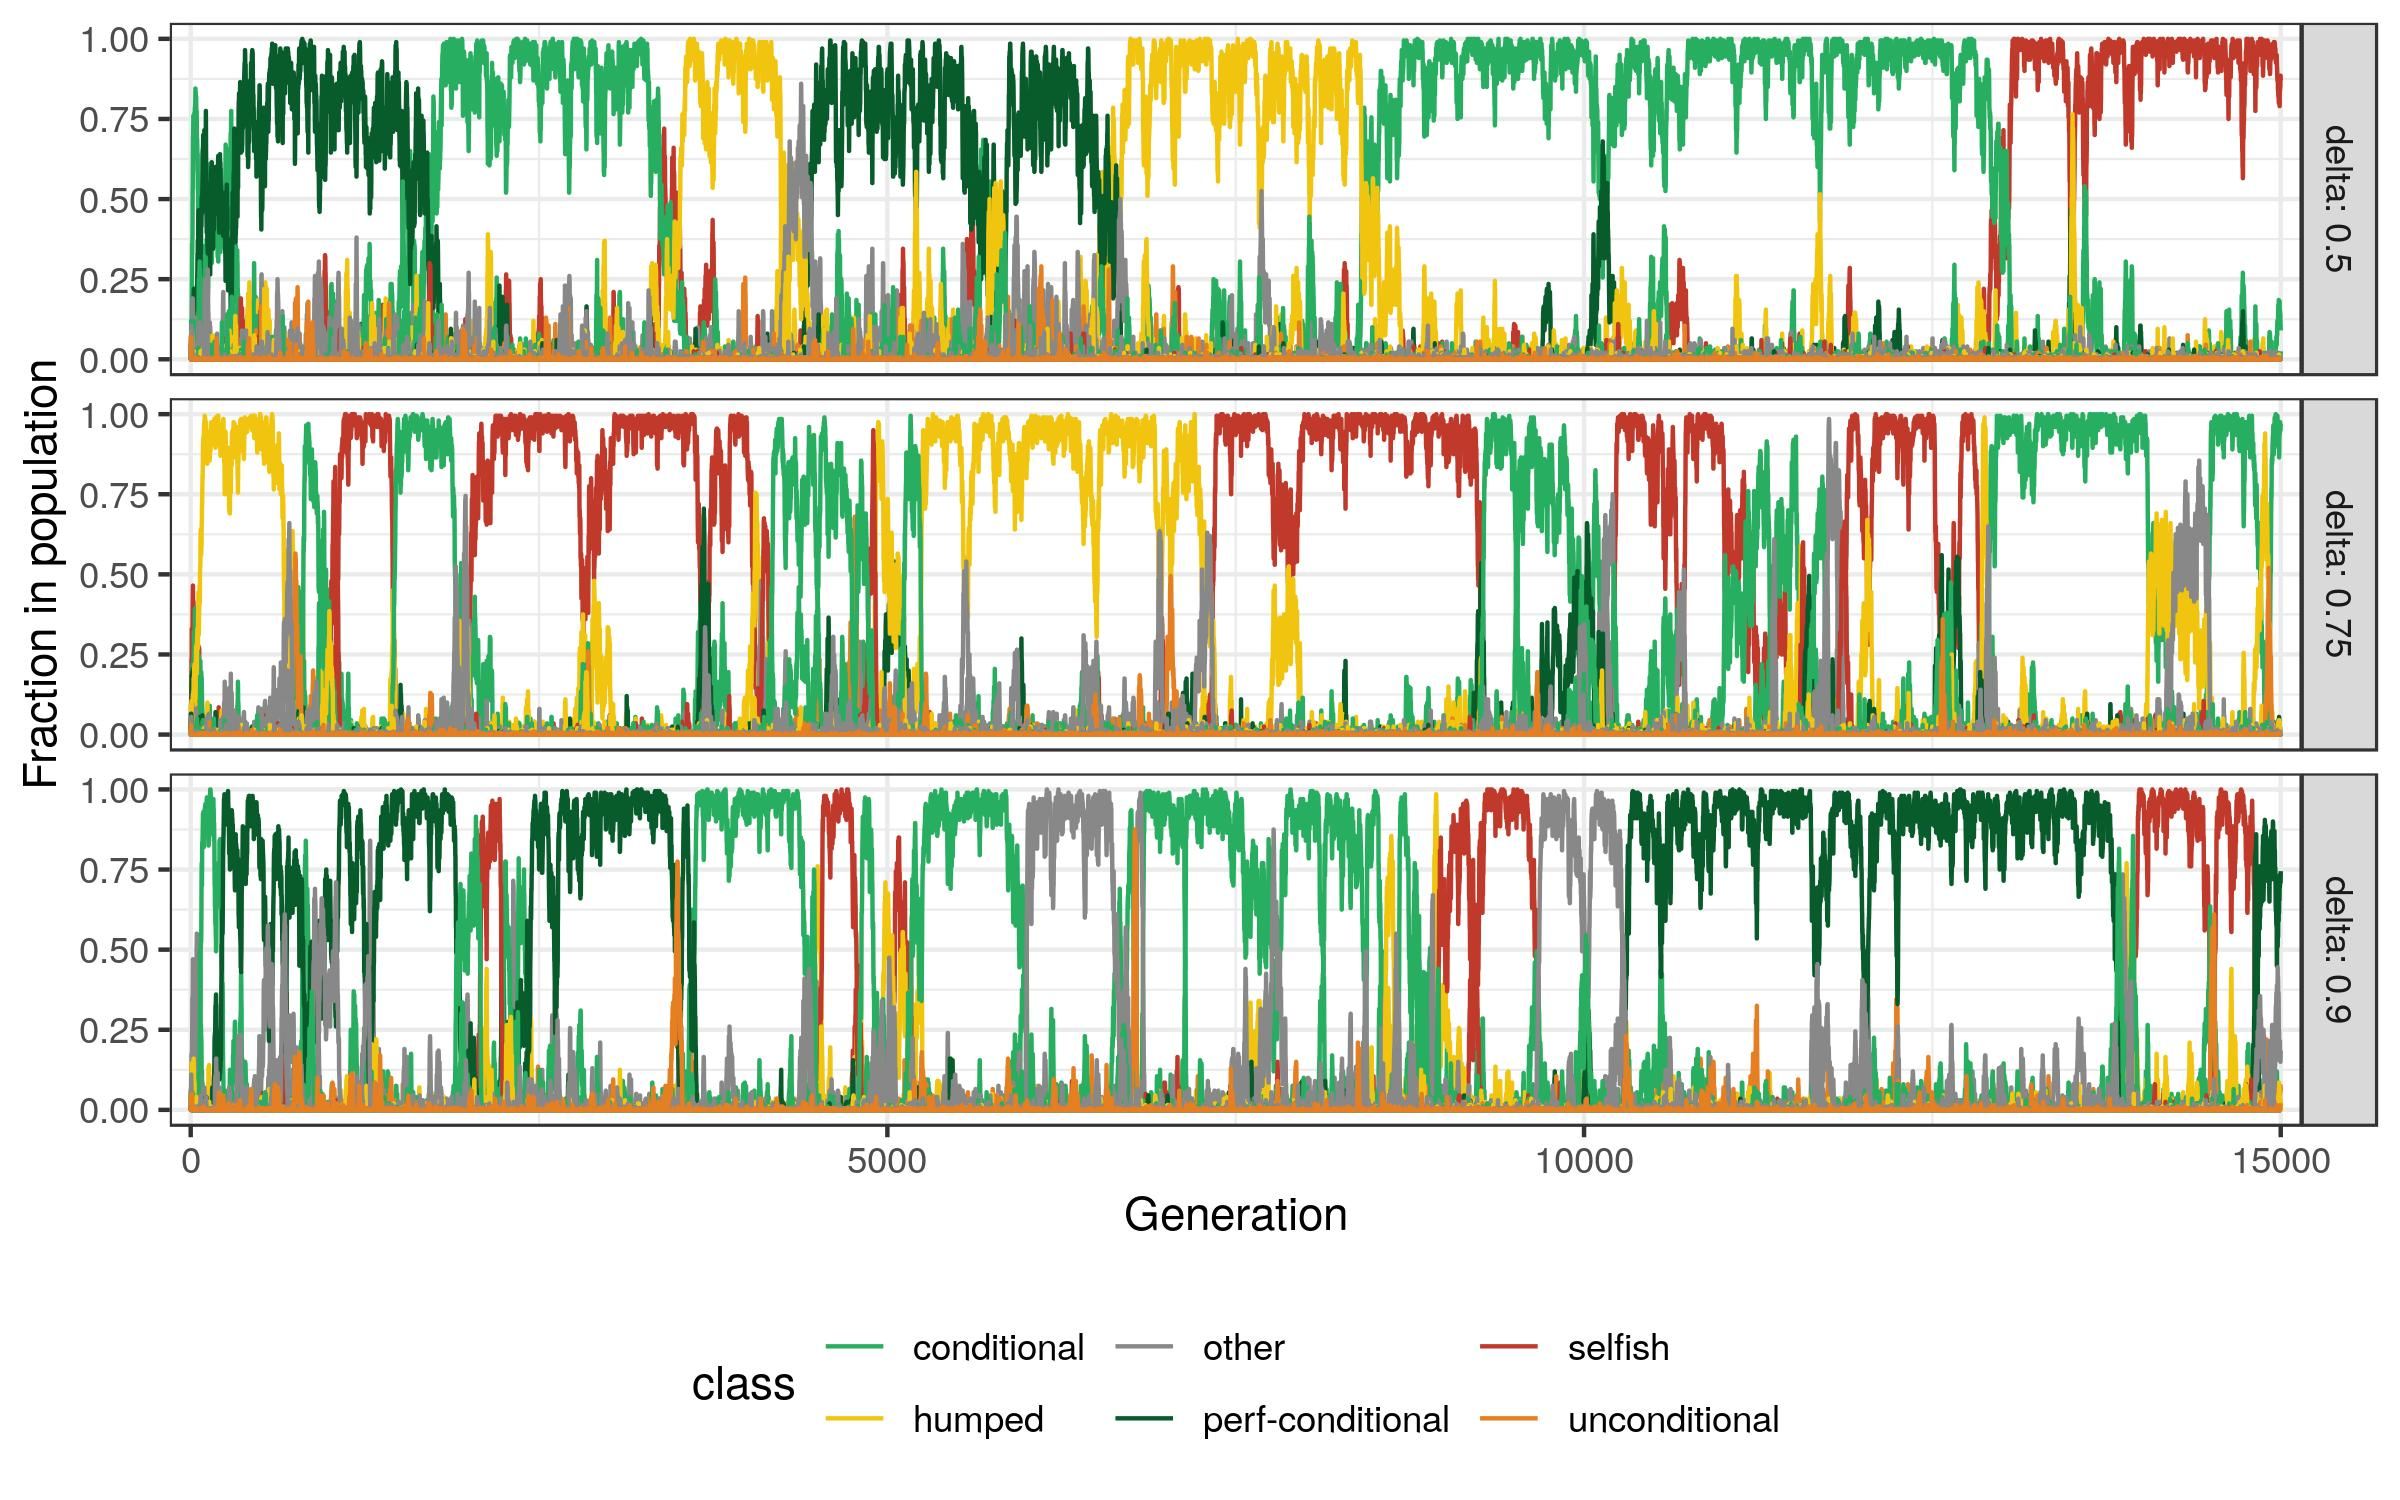
\includegraphics[width=1\linewidth]{img/types_singlerun2}
	\caption[Fraction of Strategies During Three Instances]{Fraction of Strategies During Three Instances of Simulation with Different Continuation Probabilities}
	\label{fig:evo-typessingle}
\end{figure}

\paragraph{Result 1 - Full cooperation is more likely to be obtained only at high values of continuation probability:}

\Cref{fig:evo-actionsdelta} shows the average fraction of each action; and similarly, \Cref{fig:evo-typesdelta} shows the average fraction of each type for different values of repetition probability $\delta$. Each value shown is an average of 500 simulations that ran over 5000 generations. Moreover, to reduce the effect of occasional drifts, we averaged last 2000 generations for which our simulations showed no great variation on the average values.

As $\delta$ increases, the existence probability of $M$ and $H$ gradually increases and the values of $\delta$ in which cooperation is more likely than defection is obtained only when delta is above a certain threshold. (For our parameters, $\delta > 0.75$, which is well above the theoretical threshold $c/b$. Hence, reciprocity is unlikely to promote cooperation below those values. Moreover, mid-cooperation, although being Pareto-inferior, is more likely to be obtained for those values. )

\begin{figure}[H]
	\centering
	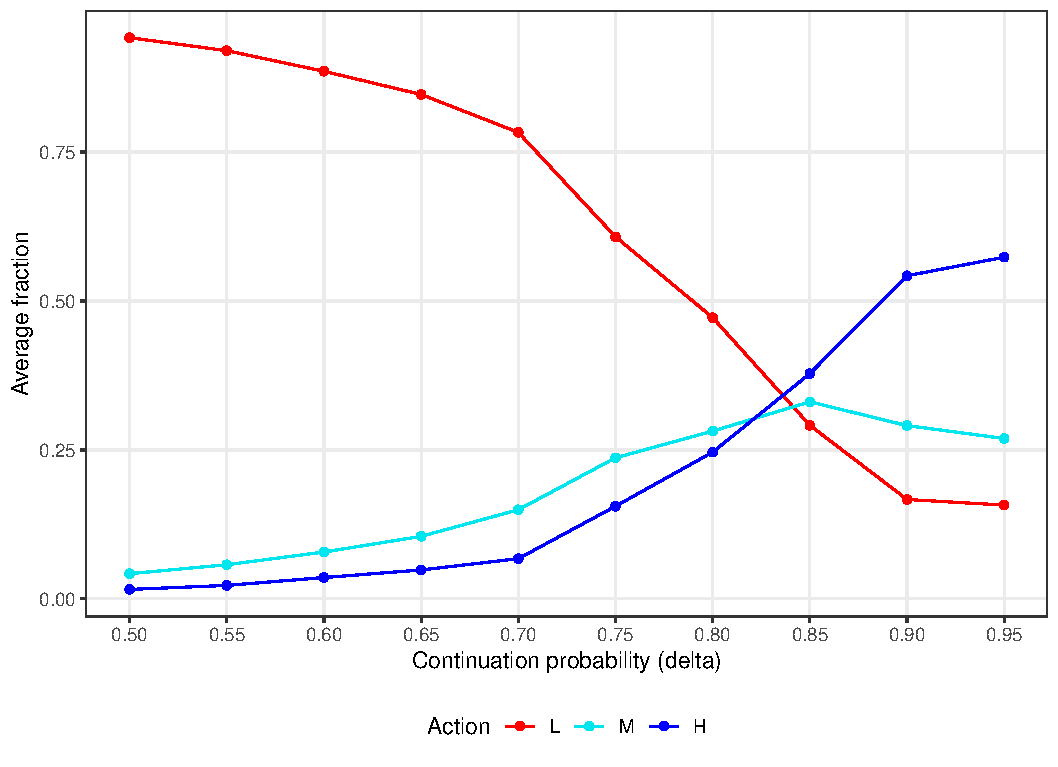
\includegraphics[width=0.7\linewidth]{img/actions_over_delta}

	\caption[Average Fraction of Actions]{Average Fraction of Actions Over 500 Repetitions for Different Values of Continuation Probability $\delta$}

	\label{fig:evo-actionsdelta}
\end{figure}

Focusing on \Cref{fig:evo-typesdelta}, we see that conditional types that are closer to selfish types are likely to exist in relatively lower values of $\delta$, though it is unlikely for them to foster cooperation, but they rather likely to survive because they are neutral mutants when defection is a the common action in the population. 



\paragraph{Result 2 - All-or-nothing cooperators are more likely to exist than perfect conditional cooperators: }

\Cref{fig:evo-typesdelta} shows that, in all continuation probabilities, all-or-nothing cooperators with an optimistic start($H-LLH$) are more likely to exist than perfect conditional cooperators ($H-LMH$). Those two types are equivalent if we remove the medium level of cooperation. In this case, they both play a tit-for-tat strategy. 

These strategies would do equally well when they play against each other in a deterministic setting: They would engage in full-cooperation($H$), which would be adventageous for both types when the conditional cooperation probability is sufficiently high.  However, when mistakes happen, all-or-nothing strategy is likely to exploit mistaken mid level cooperation($M$) by others.

\paragraph{Result 3 - Initial move of a strategy is a determinant of the success of a conditional decision:}
Consider three strategies which are identical in their responses to the counterpart, but differ in their initial move: $L-LLH$, $M-LLH$ and $H-LLH$.  All of these types, in an experimental study, would be classified as conditional cooperators. Our evidence shows that their success is highly dependent on the initial move. For instance, $L-LLH$ is relatively successful when $\delta$ is low and cooperation is unlikely. In this case, an opponent that plays $H$ is unlikely to exist in the population, and the reaction of this strategy is $L$ for all other strategies. This strategy does as good as the selfish the selfish strategy. However, agents using this strategy often fail to cooperate within each other, unless a mistake leads to high cooperation, as none of the two interacting parts initiate cooperation. The twin strategy that is successful in cooperating is $H-LMH$, but when the repetition probability is low, the first move of this strategy would cost a significant fitness that is impossible to tolerate with the cooperation within itself. When the $\delta$ is low and the  population lacks a structure that gives a higher probability for similar agents to interact, this strategy fails to survive. The strategy $M-LLH$  has strong disadvantages both where $\delta$ is low, and it is sufficiently high to sustain cooperation. 


\paragraph{Result 4 - Hump-shaped strategies are relatively successful:}
An interesting result we obtained is the relative success of hump-shaped cooperators. Such types of strategy are constantly observed in empirical studies, while the arguments regarding this type of behavior in those studies are still have been far from convincing. 

In our simulations, we have two types of humped-shaped strategies that are likely to exist: $L-LML$ and $M-LML$. The former one is relatively successful due to its proximity to selfish strategy and virtually behaving as the same as the selfish agents when no cooperation is common in the population. 

The latter one, however is a more interesting case. The reason begind the success of $M-LML$ strategy is due to its ability to coordinate in medium level of cooperation with a smaller cost than the other strategies. Moreover this strategy can exploit high-contributors as well. When the continuation probability $\delta$ is sufficient for cooperation to occur but still risky for high cooperation, this hump-shaped strategy is relatively successful.


\begin{figure}[H]
	\centering

	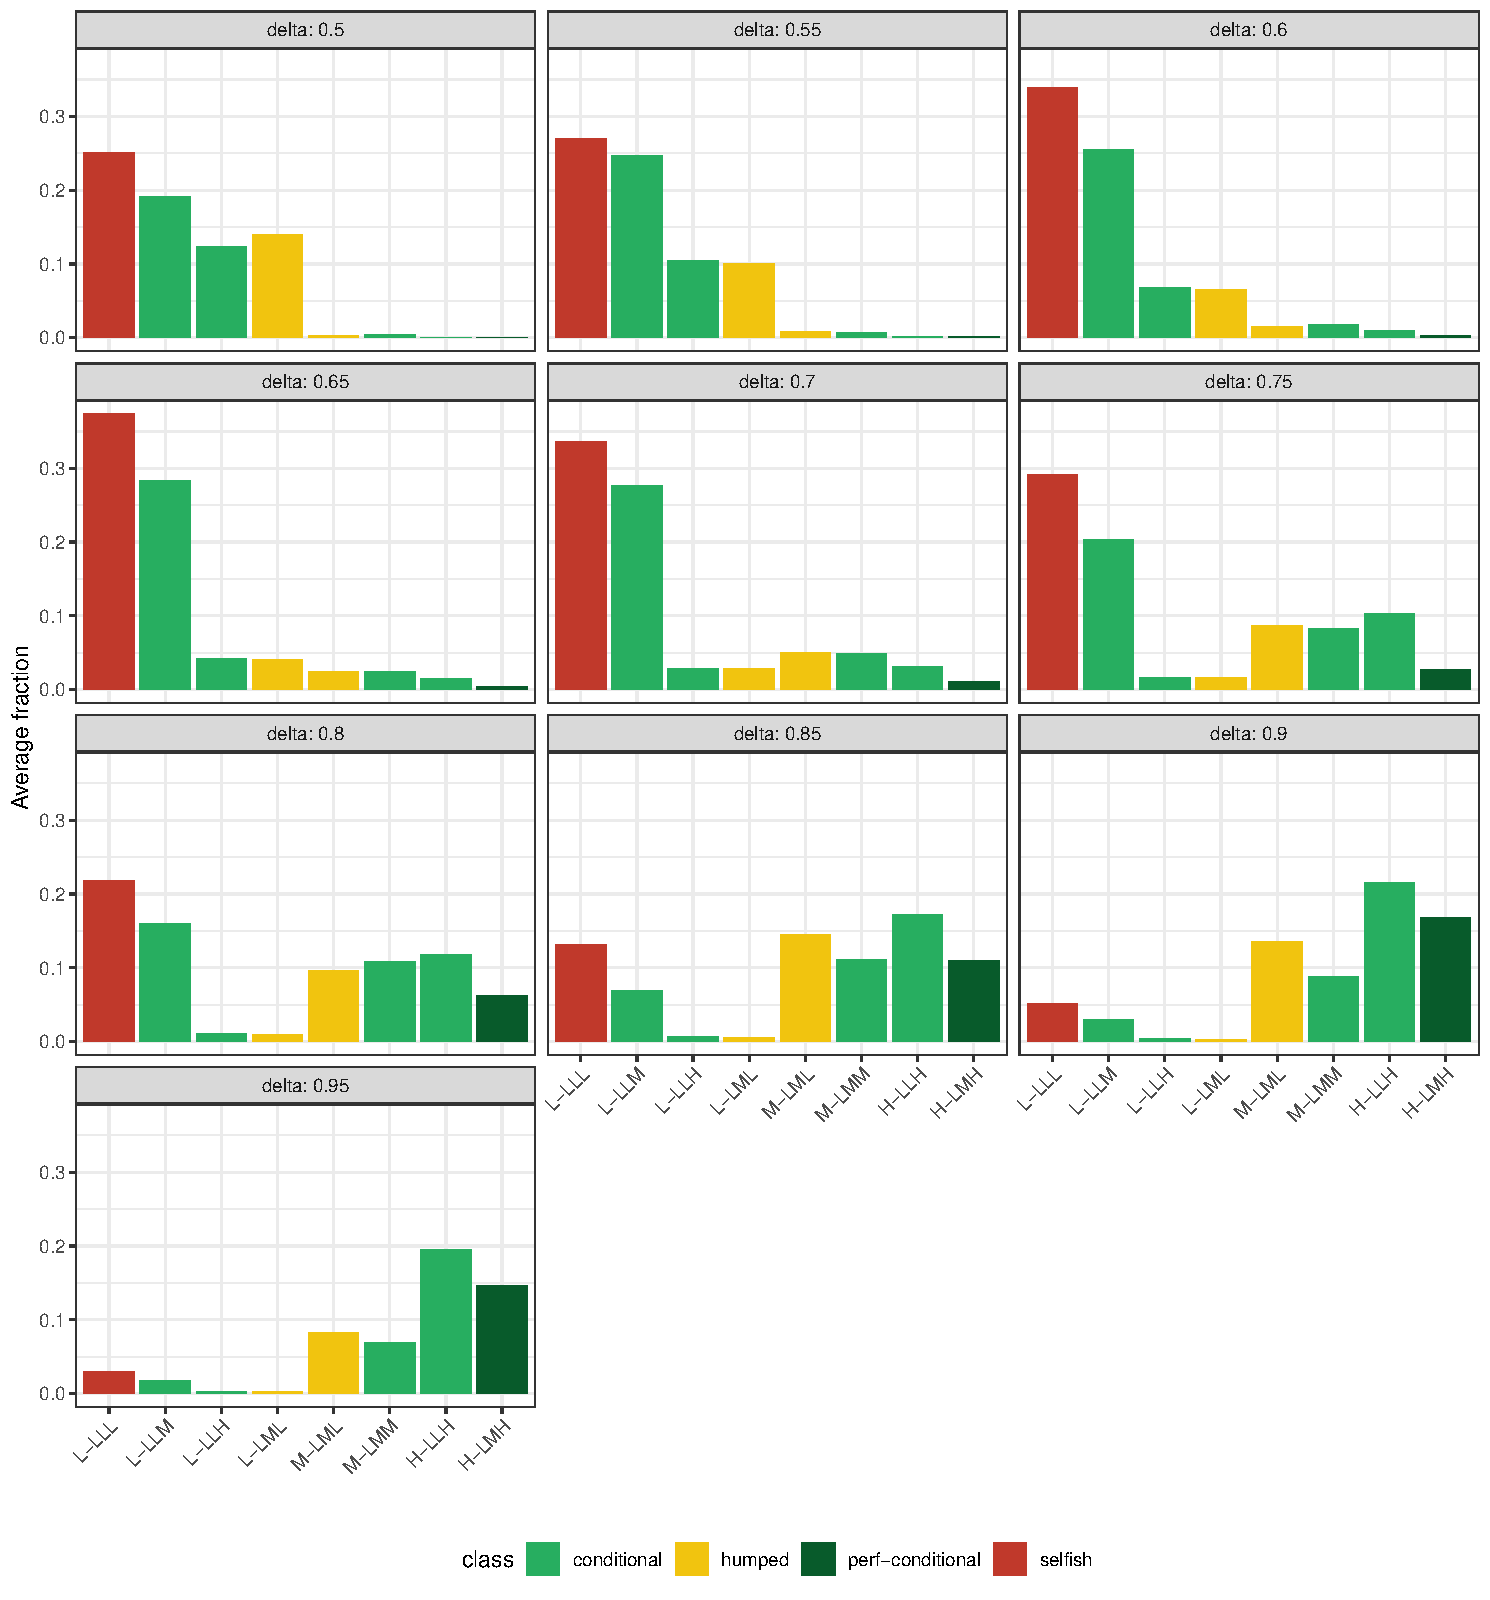
\includegraphics[width=1\linewidth]{img/types_average}

	\caption[Average Fraction of Strategies]{Average Fraction of Strategies Over 500 Repetitions for Different Values of Continuation Probability $\delta$. The Figure Includes the Strategies Which Consists at Least 10\% the Population for at Least One Delta Value.}
	\label{fig:evo-typesdelta}
\end{figure}





\section{Discussion}
 
In this study, we investigated the emergence of cooperation and relative success of conditional strategies in an extension of iterated Prionser's Dilemma. Some of the results we obtain provide supporting evidence for the previous results in a different setting. For instance, the oscillations between defection and two levels of cooperation were expected in the light of previous studies \citep{Wahl1999-nn, Nowak1989-vx, Bendor1995-zf, Imhof2005-ti, Van_Veelen2012-xf, Garcia2016-tr, Van_Veelen2012-xf}. Also, the initial strategy is indeed decisive for the success of a type \citep{Wahl1999-zi, Wahl1999-nn}. Our results suggest that the initial moves should be in accordance with the action where a strategy is most successful within itself. 


The most successful types considering all possible continuation probabilities are: selfish and relatively selfish types that start with defection($L$); hump-shaped and conditional cooperator type which has the conditional response $LMM$ that start with $M$; and all-or-nothing and perfect-conditional-cooperator types that start with $H$. Those types outperform other types who have the same conditional strategy but a different initial move. Those results suggest that strategies with a non-aligned initial move fail to reach the interaction cycle where they would profit most. 

A particularly surprising result concerns hump-shaped contributors. Those types are often observed in experiments in which conditional preferences are elicited. They are indeed the most common types after conditional cooperators and selfish types in those experiments. It is hard to rationalize this kind of strategy which can be counter-intuitive. At a first glance as they would fail fully to exploit others while not being able to cooperate at a maximum level,  but rather stuck in a medium level of cooperation. However our results suggest that as they are able to exploit mistakes made by their opponents better than the cooperative types and they do relatively better than non-cooperative types, it gives a relative advantage where the continuation probability is moderate. If we also consider the case where repetition probability changes over time, we can expect those types to do relatively better than the others. Our setup might be misleading though; since we have three levels, a monotonic increase or a monotonic decrease is not possible around the intermediate cooperation. What should one expect if there were more levels of cooperation? Possibly the answer depends on the structure of mistakes: If we assume mistaken moves to similar actions are more likely, then mistaken moves to actions that are far from the outcome of the response function,and then we might expect those monotonic increments and decreases. Due to computational complexities of this expansion creat, we seek for further research to confirm this hypothesis. 

Finally, our result might provide some explanation about the heterogeneity of conditional strategies we observe in experiments. In our setting, different type of strategies arise and different continuation probabilities: selfish types when $\delta$ is small, perfect-conditional-cooperators and all-or-none type of conditional cooperators when $\delta$ is high and  hump-shaped and imperfect conditional cooperators when delta is in-between. Though it is possibly a strong claim that those conditional preferences are direct consequences of evolution, their success in different continuation probabilities are evident. Therefore mixing individuals with different histories, either at a cultural sense or at an evolutionary sense, might result in such heterogeneity. 

%
\section{Analytical Results}
\textbf{This part was intended to take place in the chapter of Evolution of Conditional Cooperation}\\
In this section we further investigate the payoffs of the successful types of the simulations in an analytical framework. First let us describe how agents look at how agents interact. 

When two conditional strategies start to interact, the course of interaction depends on the initial move. To demonstrate lets take a look at the interaction of two perfect conditionally cooperator types that differ in their initial move: $M-LLH$ and $H-LLH$. To simplify, we will call the first strategy as ``cautious conditional cooperator'' and the second one ``generous conditional cooperator''. If the cautious type is the first mover, it starts with the strategy $M$. The response of generous type will be $L$ and they further will continue playing $L$ as long as the game continues. However if the generous type is the first mover, then the interaction starts with $H$ and the cautious type will respond with $H$ and the as the interaction goes on, both players will play $H$. As it can be seen those two types as they interact, at a certain point the strategies will go into a repetition (proof needed). This repetition can be either the same strategy as it is the case for both initial moves in our demonstration (either $L$,$L$,$L$) or it can be a cycle with different strategies played repeatedly. We will call this cycling path as the ``engagement cycle'', and the interaction happening before it starts to repeat as ``handshake interactions''. In order to calculate the total payoffs from the interaction, we need to calculate the handshake payoffs and engagement payoffs separately. 

Lets assume that both agents always cooperate in their engagement cycle and they start with cooperation. Therefore there are no handshake interaction. So the history of the game will be as the following: 
\begin{table}[H]
\begin{center}

\begin{tabular}{lccccc}
Player 1 & H &   & H &   & ... \\
Player 2 &  & H &   & H  & ...\\
\end{tabular}

\end{center}
\end{table}
then the payoffs will be;

\begin{table}[H]
\begin{center}
\begin{tabular}{lccccc}
Player 1 & -c & b  & -c & b & ...\\
Player 2 & b & -c & b  & -c  & ...\\
\end{tabular}
\end{center}
\end{table}
In that case the expected payoff for player 1 is:

\begin{align*}
E[\pi] &= \delta^0(-c)+\delta^1b+\delta^2(-c)+\delta^3b+\dots \\
       &= (-c)(\delta^0+\delta^2+\dots) + b(\delta^1+\delta^3+\dots) \\
       &= (-c) \sum_{t=0}^{\infty}\delta^{2t} + b \sum_{t=0}^{\infty}\delta^{2t+1}  \\
       &= \frac{(-c)}{1-\delta^2} + \frac{\delta b}{1-\delta^2}=\frac{(-c)+\delta b}{1-\delta^2}.
\end{align*}

The generalization is as follows: if the interaction leads us to a cycle length of four after the  $i$\textsuperscript{th} interaction,i.e. when $i$ is the size of handshake periods, and the cycle payoffs are  $a,b,c,d$ respectively, then the expected payoff from the engagement cycle for the agent would be (proof needed?):
$$E[\pi_E]=a\sum_{t=0}^{\infty}\delta^{4t+i}+b\sum_{t=0}^{\infty}\delta^{4t+i+1}+c\sum_{t=0}^{\infty}\delta^{4t+i+2}+d\sum_{t=0}^{\infty}\delta^{4t+i+3}$$
$$=\frac{a\delta^i+b\delta^{i+1}+c\delta^{i+2}+c\delta^{i+4}}{1-\delta^{i+4}}$$  

And if the engagement cycle gives the agent to the a sequence of the payoffs such as  $(x_0,x_1,\dots,x_n)$ after $i$ interactions, the expected payoff will be:
$$E[\pi_E]=\frac{\sum_{j=0}^{n}x_j\delta^{j+i}}{1-\delta^{n+1}}$$

The calculation of the expected payoffs for the handshake interactions is rather trivial. We find the path of the handshake and discound the payoffs with the delta. Then the expected payoff for an interactin will be $E[\pi] = E[\pi_H] + E[\pi_E]$.

Now we take the successful stategies and find their handshake moves and engagement cycles.


\newcommand{\me}{\textsuperscript}
\newcommand{\ot}{\textsubscript}
\newcommand{\no}{$\varnothing$}


% Payoff L-LLL
\begin{table}[H]
\setlength{\extrarowheight}{2pt}	\resizebox{1\textwidth}{!}{
\renewcommand{\arraystretch}{1.5}
 \begin{tabular}{@{}cc|cccc|cccc|c@{}}
%\toprule
         &         & \multicolumn{4}{c|}{First Mover} & \multicolumn{4}{c|}{Second Mover} &                                                                                                                                                                                       \\ \midrule
   Type  & Against & Hands.                           & Eng.cyc.                          & $\pi_H$ & $\pi_E$                     & Hands. & Eng.cyc.      & $\pi_H$ & $\pi_E$                              & $\pi_T$                                                             \\ \midrule
   L-LLL & L-LLL   & \no                              & \me{L} \ot{L}                     & -       & $\frac{\omega}{1-\delta^2}$ & \no    & \ot{L} \me{L} & -       & $\frac{\omega \delta}{1-\delta^2}$   & $\frac{1}{2}\cdot \frac{\omega}{1-\delta}$                          \\
   L-LLL & L-LLM   & \no                              & \me{L} \ot{L}                     & -       & $\frac{\omega}{1-\delta^2}$ & \no    & \ot{L} \me{L} & -       & $\frac{\omega \delta}{1-\delta^2}$   & $\frac{1}{2}\cdot \frac{\omega}{1-\delta}$                          \\
   L-LLL & L-LLH   & \no                              & \me{L} \ot{L}                     & -       & $\frac{\omega}{1-\delta^2}$ & \no    & \ot{L} \me{L} & -       & $\frac{\omega \delta}{1-\delta^2}$   & $\frac{1}{2}\cdot \frac{\omega}{1-\delta}$                          \\ 
   L-LLL & L-LML   & \no                              & \me{L} \ot{L}                     & -       & $\frac{\omega}{1-\delta^2}$ & \no    & \ot{L} \me{L} & -       & $\frac{\omega \delta}{1-\delta^2}$   & $\frac{1}{2}\cdot \frac{\omega}{1-\delta}$                          \\ 
   L-LLL & M-LML   & \no                              & \me{L} \ot{L}                     & -       & $\frac{\omega}{1-\delta^2}$ & \ot{M} & \me{L} \ot{L} & $b/2$   & $\frac{\omega \delta^2}{1-\delta^2}$ & $\frac{1}{2}\cdot\Big(\frac{b}{2} + \frac{\omega}{1-\delta}\Big)$   \\ 
   L-LLL & M-LMM   & \no                              & \me{L} \ot{L}                     & -       & $\frac{\omega}{1-\delta^2}$ & \ot{M} & \me{L} \ot{L} & $b/2$   & $\frac{\omega \delta^2}{1-\delta^2}$ & $\frac{1}{2}\cdot\Big(\frac{b}{2} + \frac{\omega}{1-\delta}\Big)$   \\
   L-LLL & H-LLH   & \no                              & \me{L} \ot{L}                     & -       & $\frac{\omega}{1-\delta^2}$ & \ot{H} & \me{L} \ot{L} & $b$     & $\frac{\omega \delta^2}{1-\delta^2}$ & $\frac{1}{2}\cdot\Big(b             + \frac{\omega}{1-\delta}\Big)$ \\
   L-LLL & H-LMH   & \no                              & \me{L} \ot{L}                     & -       & $\frac{\omega}{1-\delta^2}$ & \ot{H} & \me{L} \ot{L} & $b$     & $\frac{\omega \delta^2}{1-\delta^2}$ & $\frac{1}{2}\cdot\Big(b             + \frac{\omega}{1-\delta}\Big)$ \\

   \bottomrule
\end{tabular}
}
\caption{Interaction of type L-LLL and the relevant payoffs}
\label{tbl:evo-payoffL-LLL}
\end{table}


% Payoff L-LLM
\begin{table}[H]
\setlength{\extrarowheight}{2pt}	\resizebox{1\textwidth}{!}{
\renewcommand{\arraystretch}{1.5}
 \begin{tabular}{@{}cc|cccc|cccc|c@{}}
%\toprule
         &         & \multicolumn{4}{c|}{First Mover} & \multicolumn{4}{c|}{Second Mover} &                                                                                                                                                                                                                                                              \\ \midrule
   Type  & Against & Hands.                           & Eng.cyc.                          & $\pi_H$ & $\pi_E$                     & Hands.        & Eng.cyc.      & $\pi_H$                   & $\pi_E$                              & $\pi_T$                                                                                                           \\ \midrule
   L-LLM & L-LLL   & \no                              & \me{L} \ot{L}                     & -       & $\frac{\omega}{1-\delta^2}$ & \no           & \ot{L} \me{L} & .                         & $\frac{\omega \delta}{1-\delta^2}$   & $\frac{1}{2}\cdot \frac{\omega}{1-\delta}$                                                                        \\
   L-LLM & L-LLM   & \no                              & \me{L} \ot{L}                     & -       & $\frac{\omega}{1-\delta^2}$ & \no           & \ot{L} \me{L} & .                         & $\frac{\omega \delta}{1-\delta^2}$   & $\frac{1}{2}\cdot \frac{\omega}{1-\delta}$                                                                        \\
   L-LLM & L-LLH   & \no                              & \me{L} \ot{L}                     & -       & $\frac{\omega}{1-\delta^2}$ & \no           & \ot{L} \me{L} & .                         & $\frac{\omega \delta}{1-\delta^2}$   & $\frac{1}{2}\cdot \frac{\omega}{1-\delta}$                                                                        \\ 
   L-LLM & L-LML   & \no                              & \me{L} \ot{L}                     & -       & $\frac{\omega}{1-\delta^2}$ & \no           & \ot{L} \me{L} & .                         & $\frac{\omega \delta}{1-\delta^2}$   & $\frac{1}{2}\cdot \frac{\omega}{1-\delta}$                                                                        \\ 
   L-LLM & M-LML   & \no                              & \me{L} \ot{L}                     & -       & $\frac{\omega}{1-\delta^2}$ & \ot{M}        & \me{L} \ot{L} & $b/2$                     & $\frac{\omega \delta^2}{1-\delta^2}$ & $\frac{1}{2}\cdot\Big(\frac{b}{2} + \frac{\omega}{1-\delta}\Big)$                                                 \\
   L-LLM & M-LMM   & \no                              & \me{L} \ot{L}                     & -       & $\frac{\omega}{1-\delta^2}$ & \ot{M}        & \me{L} \ot{L} & $b/2$                     & $\frac{\omega \delta^2}{1-\delta^2}$ & $\frac{1}{2}\cdot\Big(\frac{b}{2} + \frac{\omega}{1-\delta}\Big)$                                                 \\
   L-LLM & H-LLH   & \no                              & \me{L} \ot{L}                     & -       & $\frac{\omega}{1-\delta^2}$ & \ot{H} \me{M} & \ot{L} \me{L} & $b - \delta \frac{c}{2} $ & $\frac{\omega \delta^3}{1-\delta^2}$ & $\frac{1}{2} \Big(b - \delta \frac{c}{2} + \frac{\omega}{1-\delta^3} + \frac{\omega \delta^3}{1-\delta^2}  \Big)$ \\
   L-LLM & H-LMH   & \no                              & \me{L} \ot{L}                     & -       & $\frac{\omega}{1-\delta^2}$ & \ot{H} \me{M} & \me{L} \ot{L} & $b - \delta \frac{c}{2} $ & $\frac{\omega \delta^3}{1-\delta^2}$ & $\frac{1}{2} \Big(b - \delta \frac{c}{2} + \frac{\omega}{1-\delta^3} + \frac{\omega \delta^3}{1-\delta^2}  \Big)$ \\
 \bottomrule
\end{tabular}
}
\caption{Interaction of type L-LLM and the relevant payoffs}
\label{tbl:evo-payoffL-LLM}
\end{table}




% Payoff L-LML
\begin{table}[]
\setlength{\extrarowheight}{2pt}	\resizebox{1\textwidth}{!}{
\renewcommand{\arraystretch}{1.5}
 \begin{tabular}{@{}cc|cccc|cccc|c@{}}
%\toprule
         &         & \multicolumn{4}{c|}{First Mover} & \multicolumn{4}{c|}{Second Mover} &                                                                                                                                                                                                                                                              \\ \midrule
   Type  & Against & Hands.                           & Eng.cyc.                          & $\pi_H$ & $\pi_E$                     & Hands.        & Eng.cyc.      & $\pi_H$                   & $\pi_E$                              & $\pi_T$                                                                                                           \\ \midrule
   L-LML & L-LLL   & \no                              & \me{L} \ot{L} & - & $\frac{\omega}{1-\delta^2}$ & \no           & \ot{L} \me{L} & - & $\frac{\omega \delta}{1-\delta^2}$ & - \\
   L-LML & L-LLM   & \no                              & \me{L} \ot{L} & - & $\frac{\omega}{1-\delta^2}$ & \no           & \ot{L} \me{L} & - & $\frac{\omega \delta}{1-\delta^2}$ & - \\
   L-LML & L-LLH   & \no                              & \me{L} \ot{L} & - & $\frac{\omega}{1-\delta^2}$ & \no           & \ot{L} \me{L} & - & $\frac{\omega \delta}{1-\delta^2}$ & - \\ 
   L-LML & L-LML   & \no                              & \me{L} \ot{L} & - & $\frac{\omega}{1-\delta^2}$ & \no           & \ot{L} \me{L} & - & $\frac{\omega \delta}{1-\delta^2}$ & - \\ 
   L-LML & M-LML   & \no                              & \me{L} \ot{L} & - & $\frac{\omega}{1-\delta^2}$ & \no           & \ot{M} \me{M} & - & - & - \\ 
   L-LML & M-LMM   & \no                              & \me{L} \ot{L} & - & $\frac{\omega}{1-\delta^2}$ & \no           & \ot{M} \me{M} & - & - & - \\ 
   L-LML & H-LLH   & \no                              & \me{L} \ot{L} & - & $\frac{\omega}{1-\delta^2}$ & \ot{H}        & \me{L} \ot{L} & b & - & - \\ 
   L-LML & H-LMH   & \no                              & \me{L} \ot{L} & - & $\frac{\omega}{1-\delta^2}$ & \ot{H}        & \me{L} \ot{L} & b & - & - \\ 
 \bottomrule
\end{tabular}
}
\caption{Interaction of type L-LML and the relevant payoffs}
\label{tbl:evo-payoffL-LML}
\end{table}




%%% I WAS HERE

\begin{table}[H]
\setlength{\extrarowheight}{2pt}	\resizebox{0.7\textwidth}{!}{
\renewcommand{\arraystretch}{1.5}
 \begin{tabular}{@{}cc|cc|cc@{}}
%\toprule
         &         & \multicolumn{2}{c|}{First Mover} & \multicolumn{2}{c}{Second Mover}              \\ \midrule
   Type  & Against & Hands.                           & Eng.cyc.      & Hands.        & Eng.cyc.      \\ \midrule
   L-LML & L-LLL   & \no                              & \me{L} \ot{L} & \no           & \ot{L} \me{L} \\
   L-LML & L-LLM   & \no                              & \me{L} \ot{L} & \no           & \ot{L} \me{L} \\
   L-LML & L-LLH   & \no                              & \me{L} \ot{L} & \no           & \ot{L} \me{L} \\ 
   L-LML & L-LML   & \no                              & \me{L} \ot{L} & \no           & \ot{L} \me{L} \\ 
   L-LML & M-LML   & \no                              & \me{L} \ot{L} & \no           & \ot{M} \me{M} \\ 
   L-LML & M-LMM   & \no                              & \me{L} \ot{L} & \no           & \ot{M} \me{M} \\ 
   L-LML & H-LLH   & \no                              & \me{L} \ot{L} & \ot{H}        & \me{L} \ot{L} \\ 
   L-LML & H-LMH   & \no                              & \me{L} \ot{L} & \ot{H}        & \me{L} \ot{L} \\ 
\midrule     
   M-LML & L-LLL   & \me{M}                           & \ot{L} \me{L} & \no           & \ot{L} \me{L} \\
   M-LML & L-LLM   & \me{M}                           & \ot{L} \me{L} & \no           & \ot{L} \me{L} \\
   M-LML & L-LLH   & \me{M}                           & \ot{L} \me{L} & \no           & \ot{L} \me{L} \\ 
   M-LML & L-LML   & \no                              & \me{M} \ot{M} & \no           & \ot{L} \me{L} \\ 
   M-LML & M-LML   & \no                              & \me{M} \ot{M} & \no           & \ot{M} \me{M} \\ 
   M-LML & M-LMM   & \no                              & \me{M} \ot{M} & \no           & \ot{M} \me{M} \\ 
   M-LML & H-LLH   & \me{M}                           & \ot{L} \me{L} & \ot{H}        & \me{L} \ot{L} \\ 
   M-LML & H-LMH   & \no                              & \me{M} \ot{M} & \ot{H}        & \me{L} \ot{L} \\ 
\midrule
   M-LMM & L-LLL   & \me{M}                           & \ot{L} \me{L} & \no           & \ot{L} \me{L} \\
   M-LMM & L-LLM   & \me{M}                           & \ot{L} \me{L} & \no           & \ot{L} \me{L} \\
   M-LMM & L-LLH   & \me{M}                           & \ot{L} \me{L} & \no           & \ot{L} \me{L} \\ 
   M-LMM & L-LML   & \no                              & \me{M} \ot{M} & \no           & \ot{L} \me{L} \\ 
   M-LMM & M-LML   & \no                              & \me{M} \ot{M} & \no           & \ot{M} \me{M} \\ 
   M-LMM & M-LMM   & \no                              & \me{M} \ot{M} & \no           & \ot{M} \me{M} \\ 
   M-LMM & H-LLH   & \me{M}                           & \ot{L} \me{L} & \ot{H} \me{M} & \ot{L} \me{L} \\ 
   M-LMM & H-LMH   & \no                              & \me{M} \ot{M} & \ot{H}        & \me{M} \ot{M} \\ 
 \bottomrule
\end{tabular}
}
\end{table}


\begin{table}[H]
\setlength{\extrarowheight}{2pt}	\resizebox{0.7\textwidth}{!}{
\renewcommand{\arraystretch}{1.5}
 \begin{tabular}{@{}cc|cc|cc@{}}
%\toprule
         &         & \multicolumn{2}{c|}{First Mover} & \multicolumn{2}{c}{Second Mover}       \\ \midrule
   Type  & Against & Hands.                           & Eng.cyc.      & Hands. & Eng.cyc.      \\ \midrule
   H-LLH & L-LLL   & \me{H}                           & \ot{L} \me{L} & \no    & \ot{L} \me{L} \\
   H-LLH & L-LLM   & \me{H} \ot{M}                    & \me{L} \ot{L} & \no    & \ot{L} \me{L} \\
   H-LLH & L-LLH   & \no                              & \me{H} \ot{H} & \no    & \ot{L} \me{L} \\ 
   H-LLH & L-LML   & \me{H}                           & \ot{L} \me{L} & \no    & \ot{L} \me{L} \\ 
   H-LLH & M-LML   & \me{H}                           & \ot{L} \me{L} & \ot{M} & \me{L} \ot{L} \\ 
   H-LLH & M-LMM   & \me{H} \ot{M}                    & \me{L} \ot{L} & \ot{M} & \me{L} \ot{L} \\ 
   H-LLH & H-LLH   & \no                              & \me{H} \ot{H} & \no    & \me{H} \ot{H} \\ 
   H-LLH & H-LMH   & \no                              & \me{H} \ot{H} & \no    & \me{H} \ot{H} \\ 
\midrule     
   H-LMH & L-LLL   & \me{H}                           & \ot{L} \me{L} & \no    & \ot{L} \me{L} \\
   H-LMH & L-LLM   & \me{H} \ot{M}                    & \me{L} \ot{L} & \no    & \ot{L} \me{L} \\
   H-LMH & L-LLH   & \no                              & \me{H} \ot{H} & \no    & \ot{L} \me{L} \\ 
   H-LMH & L-LML   & \me{H}                           & \ot{L} \me{L} & \no    & \ot{L} \me{L} \\ 
   H-LMH & M-LML   & \me{H}                           & \ot{L} \me{L} & \no    & \ot{M} \me{M} \\ 
   H-LMH & M-LMM   & \me{H}                           & \ot{M} \me{M} & \no    & \ot{M} \me{M} \\ 
   H-LMH & H-LLH   & \no                              & \me{H} \ot{H} & \no    & \me{H} \ot{H} \\ 
   H-LMH & H-LMH   & \no                              & \me{H} \ot{H} & \no    & \me{H} \ot{H} \\ 



 \bottomrule
\end{tabular}
}
\end{table}

\begin{sidewaystable}[H] % <-- HERE
\centering
\def\arraystretch{2}%  1 
\resizebox{\textwidth}{!}{
\begin{tabular}{|C{1.5cm}| C{4cm}|C{4cm}|C{4cm}|C{4cm}|C{4cm}|C{4cm}|C{4cm}|C{4cm}| }\hline
       & L-LLL & L-LLM & L-LLH & L-LML & M-LML & M-LMM & H-LLH & H-LMH \\ \hline 
L-LLL  & $\frac{1}{2}\cdot \frac{\omega}{1-\delta}$ & $\frac{1}{2}\cdot \frac{\omega}{1-\delta}$ & $\frac{1}{2}\cdot \frac{\omega}{1-\delta}$ & $\frac{1}{2}\cdot \frac{\omega}{1-\delta}$  & $\frac{1}{2}\cdot\Big(\frac{b}{2} + \frac{\omega}{1-\delta}\Big)$ & $\frac{1}{2}\cdot\Big(\frac{b}{2} + \frac{\omega}{1-\delta}\Big)$  &
$\frac{1}{2}\cdot\Big(b             + \frac{\omega}{1-\delta}\Big)$ & $\frac{1}{2}\cdot\Big(b             + \frac{\omega}{1-\delta}\Big)$ \\
 L-LLM & $\frac{1}{2}\cdot \frac{\omega}{1-\delta}$ & $\frac{1}{2}\cdot \frac{\omega}{1-\delta}$ & $\frac{1}{2}\cdot \frac{\omega}{1-\delta}$ & $\frac{1}{2}\cdot \frac{\omega}{1-\delta}$ & $\frac{1}{2}\cdot\Big(\frac{b}{2} + \frac{\omega}{1-\delta}\Big)$ & $\frac{1}{2}\cdot\Big(\frac{b}{2} + \frac{\omega}{1-\delta}\Big)$ & $\frac{1}{2} \Big(b - \delta \frac{c}{2} + \frac{\omega}{1-\delta^3} + \frac{\omega \delta^3}{1-\delta^2}  \Big)$ & $\frac{1}{2} \Big(b - \delta \frac{c}{2} + \frac{\omega}{1-\delta^3} + \frac{\omega \delta^3}{1-\delta^2}  \Big)$ \\
 L-LLH &       &       &       &       &       &       &       &       \\ 
 L-LML &       &       &       &       &       &       &       &       \\ 
 M-LML &       &       &       &       &       &       &       &       \\ 
 M-LMM &       &       &       &       &       &       &       &       \\ 
 H-LLH &       &       &       &       &       &       &       &       \\ 
 H-LMH & & & & & &  & &                                                                \\ \hline 
\end{tabular}
}
\caption{Payoff table of the supergame}
\end{sidewaystable} % <-- HERE

% Finally in our discussion, we can exploit of the information we have from our experiment in \Cref{chap:stability}. The stage game in our simulation is similar to the game subjects play in each interaction. Surprisingly most of the strategies that are successful in our simulations are strategies that either intuitively make sense or observed in the experiment. However, the most successful strategy when $\delta$ is high, $H-LLH$ is a strategy that is not frequently observed in the population. That possibly requires more interpretation which we are not able to provide in this paper.




% The term \textit{reciprocal altrism} was coined by biologist \citet{Trivers1971}. Trivers  To formally describe, for reciprocal altruism to arise, the conditoin $\delta > c/b$ has to be satisfied, where $\delta$ denotes iprobability of re-interaction with the other, $c$ denotes the cost of the aid, and $b$ the benefit of the aid to other person.



%%% Local Variables:
%%% mode: latex
%%% TeX-master: "../main"
%%% End:

\appendix
%\section{Additional Material: Stability of Conditional Cooperation}
\label{chap:appx-evo}

\section{Type Definitions}

\begin{table}[ht]
\centering
 \resizebox{0.6\textwidth}{!}{
\begin{tabular}{|lll|c|lll|}
  \hline
 & denotion & classification & & & denotion & classification \\ 
  \hline
  0 & L-LLL & selfish &  &   41 & M-MMH & conditional \\ 
  1 & L-LLM & conditional &  &   42 & M-MHL & humped \\ 
  2 & L-LLH & conditional &  &   43 & M-MHM & humped \\ 
  3 & L-LML & humped &  &   44 & M-MHH & conditional \\ 
  4 & L-LMM & conditional &  &   45 & M-HLL & other \\ 
  5 & L-LMH & perf-conditional &  &   46 & M-HLM & other \\ 
  6 & L-LHL & humped &  &   47 & M-HLH & other \\ 
  7 & L-LHM & humped &  &   48 & M-HML & other \\ 
  8 & L-LHH & conditional &  &   49 & M-HMM & other \\ 
  9 & L-MLL & other &  &   50 & M-HMH & other \\ 
  10 & L-MLM & other &  &   51 & M-HHL & other \\ 
  11 & L-MLH & other &  &   52 & M-HHM & unconditional \\ 
  12 & L-MML & other &  &   53 & M-HHH & unconditional \\ 
  13 & L-MMM & unconditional &  &   54 & H-LLL & selfish \\ 
  14 & L-MMH & conditional &  &   55 & H-LLM & conditional \\ 
  15 & L-MHL & humped &  &   56 & H-LLH & conditional \\ 
  16 & L-MHM & humped &  &   57 & H-LML & humped \\ 
  17 & L-MHH & conditional &  &   58 & H-LMM & conditional \\ 
  18 & L-HLL & other &  &   59 & H-LMH & perf-conditional \\ 
  19 & L-HLM & other &  &   60 & H-LHL & humped \\ 
  20 & L-HLH & other &  &   61 & H-LHM & humped \\ 
  21 & L-HML & other &  &   62 & H-LHH & conditional \\ 
  22 & L-HMM & other &  &   63 & H-MLL & other \\ 
  23 & L-HMH & other &  &   64 & H-MLM & other \\ 
  24 & L-HHL & other &  &   65 & H-MLH & other \\ 
  25 & L-HHM & unconditional &  &   66 & H-MML & other \\ 
  26 & L-HHH & unconditional &  &   67 & H-MMM & unconditional \\ 
  27 & M-LLL & selfish &  &   68 & H-MMH & conditional \\ 
  28 & M-LLM & conditional &  &   69 & H-MHL & humped \\ 
  29 & M-LLH & conditional &  &   70 & H-MHM & humped \\ 
  30 & M-LML & humped &  &   71 & H-MHH & conditional \\ 
  31 & M-LMM & conditional &  &   72 & H-HLL & other \\ 
  32 & M-LMH & perf-conditional &  &   73 & H-HLM & other \\ 
  33 & M-LHL & humped &  &   74 & H-HLH & other \\ 
  34 & M-LHM & humped &  &   75 & H-HML & other \\ 
  35 & M-LHH & conditional &  &   76 & H-HMM & other \\ 
  36 & M-MLL & other &  &   77 & H-HMH & other \\ 
  37 & M-MLM & other &  &   78 & H-HHL & other \\ 
  38 & M-MLH & other &  &   79 & H-HHM & unconditional \\ 
  39 & M-MML & other &  &   80 & H-HHH & unconditional \\ 
  40 & M-MMM & unconditional &  &  & & \\ \hline 
\end{tabular}
}
\caption{All Possible Types and Their Classifications}
\label{tbl:evo-alltypes}
\end{table}



\section{Additional Data}
\label{sec:evo-additional}
\begin{figure}[H]
\begin{center}
    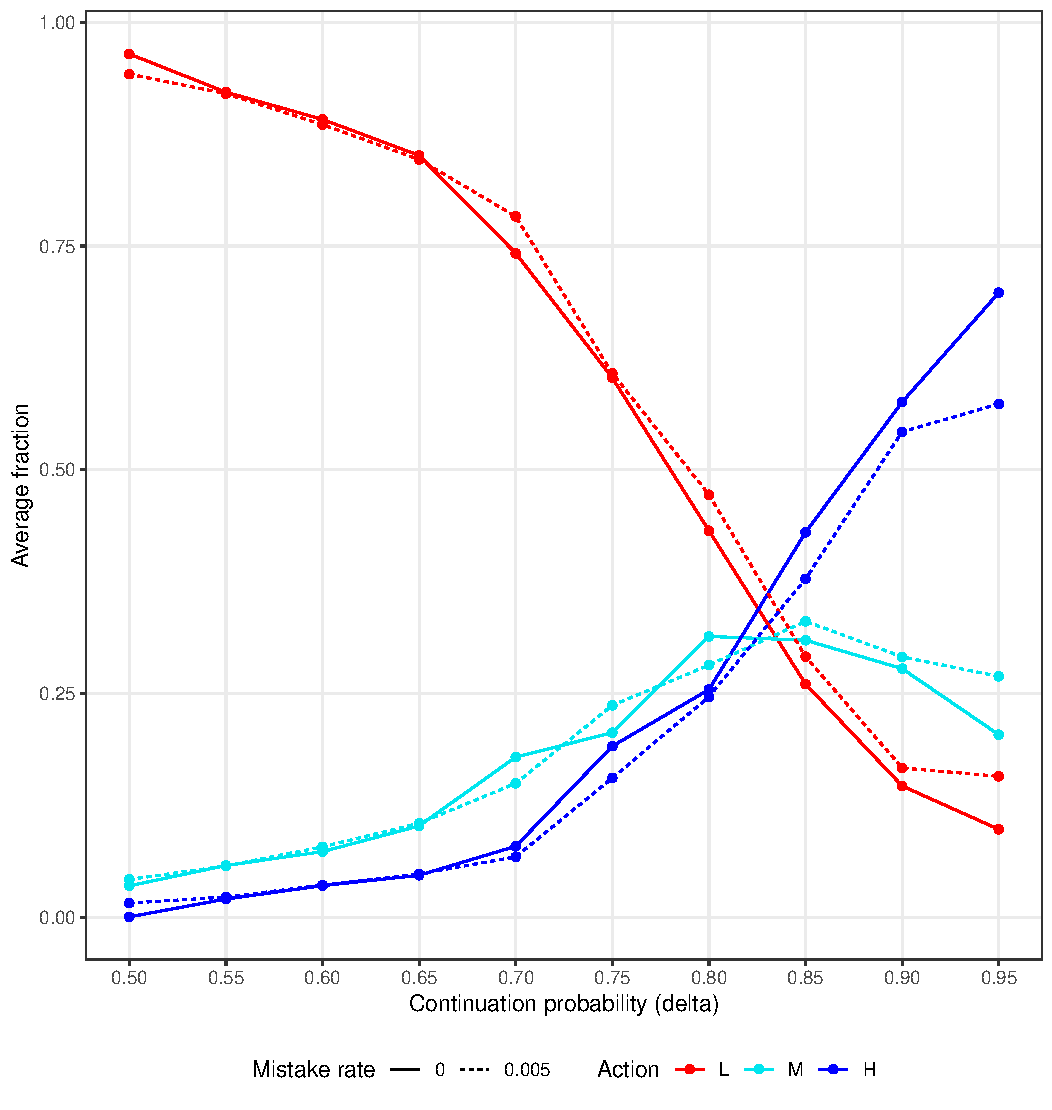
\includegraphics[width=0.8\linewidth]{img/actions_over_delta_with_mistakes.pdf}
    \caption{Comparison of Actions with and without mistakes.}
	\label{fig:mistake-comparision}
\end{center}
\end{figure}


\begin{figure}[H]
\begin{center}
    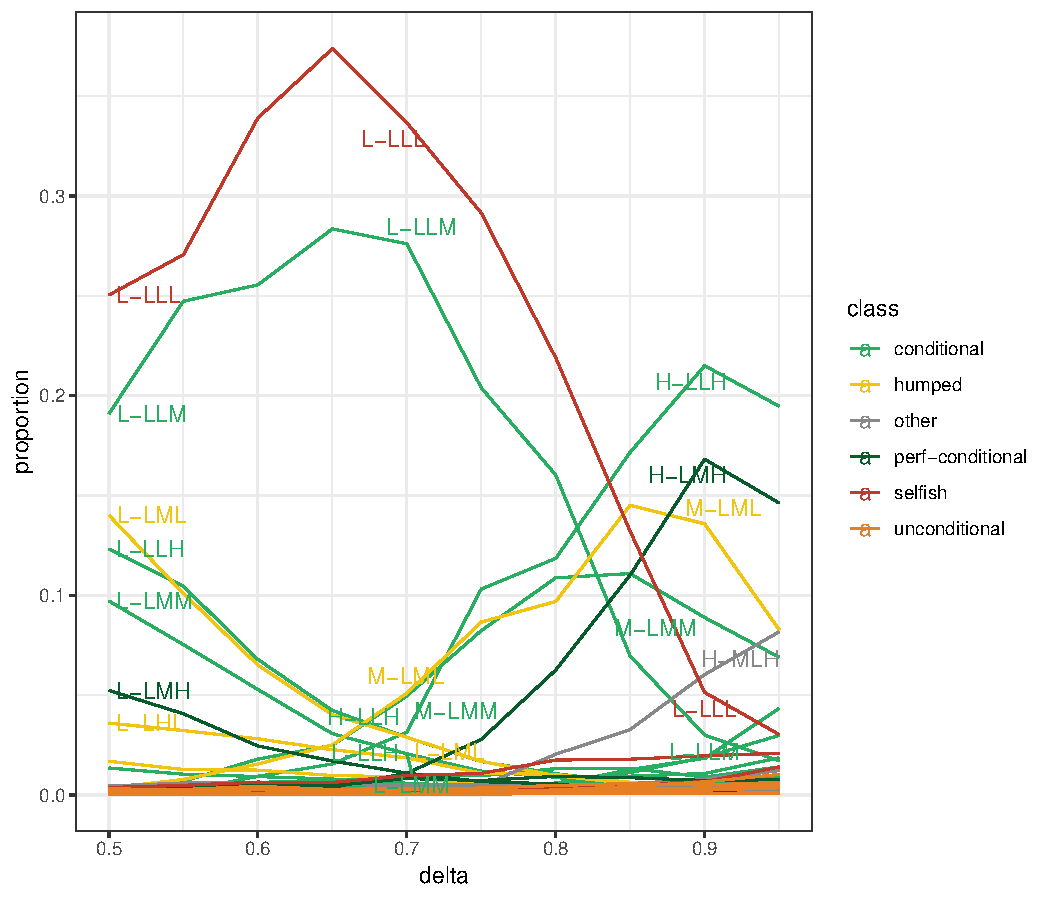
\includegraphics[width=0.8\linewidth]{img/all_types_t05.pdf}
    \caption{All types' performance for different continuation probabilities.}
	\label{fig:alltypes}
\end{center}
\end{figure}


%%% Local Variables:
%%% mode: latex
%%% TeX-master: "../main"
%%% End:



%next line adds the Bibliography to the contents page
\addcontentsline{toc}{chapter}{Bibliography}
%uncomment next line to change bibliography name to references
%\renewcommand{\bibname}{References}
%\bibliography{refs}        %use a bibtex bibliography file refs.bib
%\bibliographystyle{plain}  %use the plain bibliography style
\bibliographystyle{apalike}  
\bibliography{./thesis}  
\end{document}

